% !TeX root = ../../main.tex
\section{Smart Device}\label{section:smart-device}

The \enquote{Smart Device} is a part of the \ac{UBII} front end. Because it is web-based, only data which is available through the \textbf{Web \acp{API}} can be obtained. Since it was not designed for a specific use case, it is thought as general purpose or testing device. Only touch positions, touch events, orientation and acceleration is sent to different topics using the \textbf{\ac{UBII} Client}. For more specific scenarios, the smart device can not be used and a custom interface has to be implemented. For the experiments in this thesis though, the smart device client was sufficient, after implementing some improvements.

The data which is published, is also displayed on the screen for debugging purposes. It is possible to set the view in full screen mode, to prevent unintentional interactions with control elements of the web browser or the operating system. Since the reference system for the orientation is fixed to the earth~\cite[Chapter~4.1]{DevicesandSensorsWorkingGroup.2019}, a calibration system was implemented. With the press of the \enquote{Calibrate} button, the device is calibrated to the new orientation.

The orientation is provided by the \textbf{Web API} through the \lstinline{DeviceOrientation} event. % 
% describe orientational comes from the imu, 
%is interpolated, 
%but has limitations actually list limitations
%but is enough

% note that it coul;d be derived from the gravitional vector and geometry.

% maybe show listing of device smart device register



% extend grafic um gamma and beta value, make smaller
\begin{figure}[htpb]
  \centering
  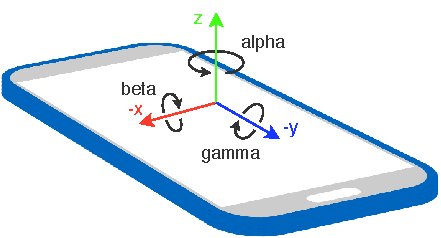
\includegraphics[width=12cm]{figures/webapi_device_orientation.pdf}
  \caption[Device Orientation]{The specification of the orientation values visualized. The $x$ and $y$ axes are inverted for the sake of clarity.}\label{fig:ubii_front_end}
\end{figure}


% why did i use it for this thesis?